\section{Архитектура и проектирование приложения}
\label{sec:arch_and_mod}
 
\subsection{Компоненты и Flux}
Так как для разработки был выбран ReactJS, то при разработке было решено придерживаться характерных для данной библиотеки архитектурных подходов.
React использует компонентно-ориентированную архитектуру. 
Она заключается в том, что визуальное представление, данные, от которых зависит пользовательский интерфейс, и логика интерфейса выносятся в единую сущность~--- компонент. 
Данный подход можно сравнить с MVC. 
Отличие заключается в том, что только V - View полностью представлен в компонентно-ориентированной архитектуре.
Задачи Model и Controller, которые непосредственно связаны с View, перенесены в компонент.
 
Для того, чтобы заполнить пробелы компонентно-ориентированной архитектуры, компания Facebook предлагает использовать вместе с React такой архитектурный подход, как Flux. 
Схема данных архитектур представлена на рисунке~\ref{fig:arch:flux}.
 
\begin{figure}[H]
 \centering
   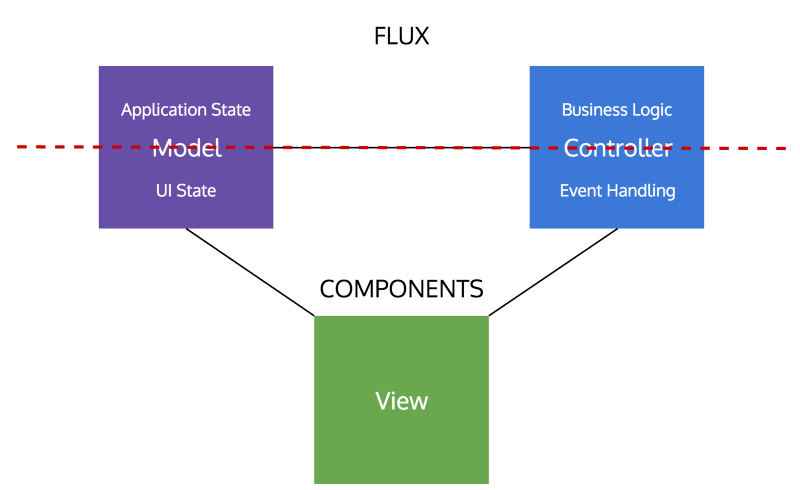
\includegraphics[scale=0.5]{flux.png} 
   \caption{Flux и компонентно-ориентированная архитектура}
   \label{fig:arch:flux}
\end{figure}
 
Главной особенностью Flux является односторонняя направленность передачи данных между компонентами Flux-архитектуры. 
Данный подход делает поток данных предсказуемым и позволяет легче производить тестирование и поиск ошибок. 
Flux-архитектура содержит три основных слоя:
\begin{itemize}
 \item action (действие);
 \item store (хранилище);
 \item view (представление).
\end{itemize}
 
Действие представляет собой набор из имени и необязательной полезной нагрузки. 
Хранилище является источником состояния приложения, который при получении действий обновляет своё состояние. 
Состояние из хранилища используется представлениями для презентации информации пользователю. 
Популярной библиотекой реализующей Flux-архитектуру является Redux\cite{redux}. 
Она используется в данном проекте для реализации Flux\hyphархитектуры.
 
\subsection{Serverless архитектура}
Serverless-вычисления (бессерверные-вычисления) - модель облачных вычислений, в которых платформа динамически руководит выделением вычислительных ресурсов. 
В данном случае бессерверный не означает отсутствие сервера как такового, под этим понимается то, что пользователю конкретной платформы не нужно заниматься созданием и настройкой собственного сервера. 
Данный подход позволяет значительно сэкономить ресурсы и уменьшить срок разработки, так как многие важные аспекты серверной части на себе берёт платформа. 
В рамках данного проекта такой платформой выступает Firebase.
 
\subsection{Организация и описание модулей приложения}
Разработанное веб-приложение можно разделить на три составляющие:
\begin{itemize}
 \item Клиентское приложения на ReactJS;
 \item Модуль Firebase для работы с базой данных;
 \item API cервер для обработки запросов;
\end{itemize}
 
Клиентское приложение является основным модулем для данного проекта. В рамках клиентского приложения реализованы основные функциональные возможности данного проекта:
\begin{itemize}
 \item создание профиля пользователя и управление пользовательскими данными;
 \item просмотр и поиск доступных комнат;
 \item создание комнаты;
 \item подключение к комнате;
 \item управление воспроизведением при помощи плеера.
\end{itemize}
 
Модуль Firebase отвечает за управление данными, их организацию и процесс передачи данных клиентскому приложению и Python сервису. Также Firebase используется для авторизации и управления пользователями и их данными.
 
Python сервис представляет из себя API сервер, основная функция которого заключается в обработке текста, который пользователь вводит при добавлении видео в текущую комнату. Сервер, анализируя полученные данные, старается найти подходящий вариант видеоролика среди поддерживаемых сервисов. Для ускорения выдачи результатов в будущем, часть данных сохраняется в Firebase.
 
На рисунке~\ref{fig:arch:modules_scheme} изображена схема взаимодействия вышеперечисленных модулей.
 
\begin{figure}[H]
 \centering
   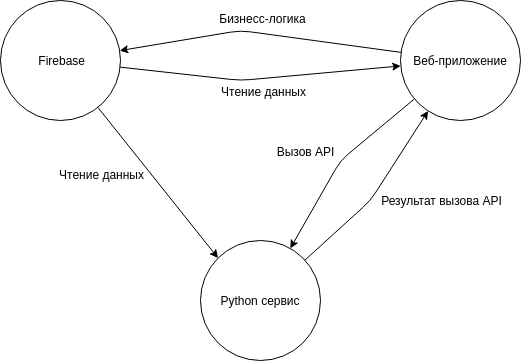
\includegraphics[scale=0.8]{modules.png} 
   \caption{Структура модулей приложения}
   \label{fig:arch:modules_scheme}
\end{figure}
 
\subsection{Описание сущностей данных}
Любое приложение используется для взаимодействия с данными, это может быть как работа с определёнными документами, так данные и сущности необходимы для реализации бизнес-логики.
Рассмотрим основные сущности данных, их организацию и связи, необходимы для работы веб-приложения. Для организации данных используется несколько ключевых коллекций:
\begin{itemize}
 \item rooms;
 \item roominfo;
 \item playlists;
 \item messages.
\end{itemize}
 
Так управление пользователями осуществляет Firebase, то как таковой модели данных для неё не требуются, но для полноты картины ниже представлена структура модели пользователя:
\begin{itemize}
 \item uid (тип строки, уникальный идентификатор пользователя);
 \item displayName (тип строки, произвольное имя пользователя);
 \item email (тип строки, электронный адрес пользователя).
\end{itemize}
 
\subsubsection{Коллекция rooms}~\par
Данная коллекция содержит документы, которые необходимы для синхронизации состояния воспроизведения у разных клиентских приложений. Основная информация, которая описывает состояние видеоролика, это:
\begin{itemize}
 \item источник текущего видеоролика;
 \item время текущего видеоролика;
 \item состояние воспроизведения (на паузе видео или нет).
\end{itemize}
 
Исходя из необходимого набора данных, документы коллекции rooms имеют три поля:
\begin{itemize}
 \item src (имеет тип строки, хранит ссылку на источник видеофайла);
 \item time (имеет тип числа, хранит текущее время видео в секундах);
 \item paused (имеет булевый тип, если true, то видео должно быть на паузе и наоборот).
\end{itemize}
 
\subsubsection{Коллекция roominfo}~\par
Данная коллекция служит для объединения информации характерной для сущности комнаты, которая необходима для её идентификации и поиска. Среди доступных полей имеются:
\begin{itemize}
 \item name (имеет тип строки, содержит название комнаты);
 \item hasPassword (имеет булевый тип, используется для отображения формы для ввода пароля при входе в комнаты, если имеет значение true);
 \item password (имеет тип строки, хранит в себе пароль указанный пользователем при создании комнаты).
\end{itemize}
 
\subsubsection{Коллекция playlists}~\par
\label{arch:data:playlist}
Данная коллекция хранит документы, которые являются представлением текущего списка видеороликов для конкретной комнаты. Документы данной коллекции имеют следующую структуру:
\begin{itemize}
 \item videos (имеет тип массива, который содержит объекты, которые описывают сущность видеоролика).
\end{itemize}
 
У объектов видеороликов нет представления в виде документов, но эта структура данных крайне важна, так как в ней содержатся основные данные необходимые для воспроизведения и идентификации видеоролика. Данный объект имеет следующую структуру:
\begin{itemize}
 \item name (имеет тип строки, содержит название видеоролика);
 \item src (имеет тип словаря, содержит набор пар ключ значение для различных источников данного видео);
 \item userInput (имеет тип строки, содержит значение, при помощи которого был добавлен видеоролик).
\end{itemize}
 
\subsubsection{Коллекция messages}~\par
Данная коллекция содержит документы, которые являются представлением пользовательского чата конкретной комнаты. Документы данной коллекции имеют следующую структуру:
\begin{itemize}
 \item messages (имеет тип массива, который содержит объекты, которые описывают сущность сообщения).
\end{itemize}
 
Объекты сообщения похожи по своей сути на объекты видео из подраздела~\ref{arch:data:playlist}. Данные объекты имеют следующую структуру:
\begin{itemize}
 \item username (имеет тип строки, содержит имя пользователя, отображаемое в чате);
 \item userId (имеет тип строки, содержит уникальный идентификатоп пользователя);
 \item message (имеет тип строки, содержит пользовательское сообшение отправленное в чат)
 \item date (имеет тип даты, содержит дату отправления сообщения пользователем);
\end{itemize}
 
\subsubsection{Организация документов из разных коллекций}~\par
Документы в перечисленных коллекциях не содержат явного идентификатора комнаты среди своих полей, это вызвано тем, что у каждого документа коллекции должен быть уникальный для неё идентификатор, по которому можно обратиться к документу. 
При создании комнаты в первую очередь происходит инициализация документа из коллекции roominfo. 
Новому документу в качестве идентификатора ставится сгенерированный UUID. 
При удачном создании этого документа, происходит создание документов в других коллекциях (эти документы будут иметь такой же уникальный идентификатор).
 
Благодаря этому после получения списка идентификаторов комнат, мы имеем возможность получить необходимую в данный момент информацию из необходимой коллекции по известному идентификатору. 
Это сделано для минимизации данных, которые пользователю придётся получать с сервера во время синхронизации видео.
Структура документов и их связи представлена на рисунке~\ref{fig:arch:docs_connections}.
 
\begin{figure}[H]
 \centering
   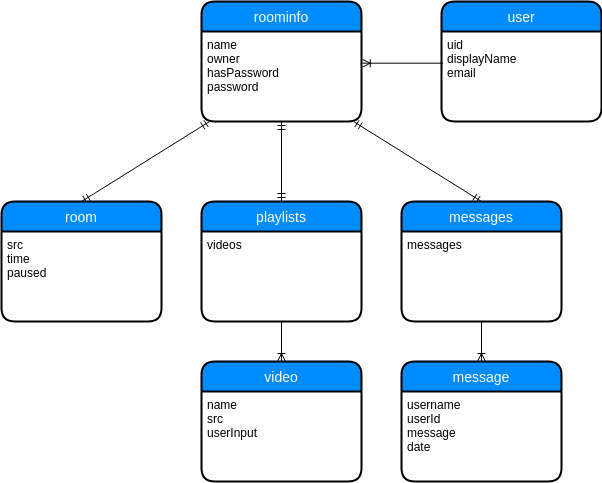
\includegraphics[scale=0.5]{data.png} 
   \caption{Структура данных}
   \label{fig:arch:docs_connections}
\end{figure}
 
\subsection{API сервер}
Изначально стояла задача разработать веб-приложение без написания собственного сервера, это позволило бы снизить трудозатраты на разработку и дальнейшую поддержку. Однако в ходе проектирования выяснилось, что реализовать возможность по поиску видео без использования сервера невозможно из-за ограничений сторонних видеосервисов. Из-за данного ограничения было решено разработать вспомогательный API cервер на языке Python. Данный сервер нужен для обработки информации и выполнения операций, которые невозможно выполнить при помощи Firebase или в самом веб\hyphприложении.
 
На данный момент его единственная задача заключается в том, чтобы обработать текст введённый пользователем при добавлении видео в список воспроизведения.
Затем ему необходимо определить то, чем является введенные данные: текстом или ссылкой. 
Если данные являются ссылкой на страницу содержащую видеоролик и наше веб-приложение поддерживает данный видеосервис, сервер запрашивает информацию о видео напрямую с видеосервиса, если такая возможность доступна. 
В противном случае сервер старается получить данную информации другими способами (Для YouTube необходима сторонний модуль для Python youtube-dl). 
Если введенные пользователем данные являются текстом, происходит поиск по данному тексту на поддерживаемых видеосервисах.
При нахождении подходящего видеоролика, данные полученные от видесервиса преобразуются в формат, который использует веб-приложение.
Эти данные должны соответствовать структуре описанной в подразделе~\ref{arch:data:playlist}. 
После преобразования данных они отправляются обратно клиенту в формате JSON. 
Схема алгоритма по обработке пользовательского запроса представлена на рисунке~\ref{fig:arch:python_service}.
 
\begin{figure}[H]
 \centering
   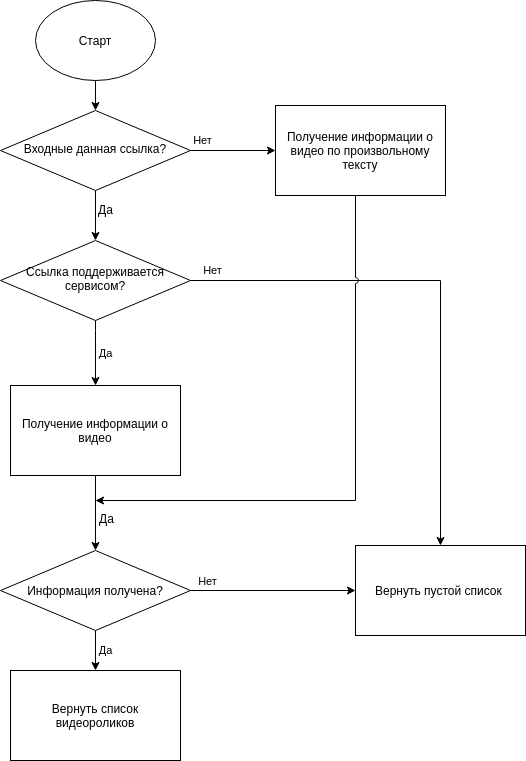
\includegraphics[scale=0.5]{python.png} 
   \caption{Алгоритм поиска видео}
   \label{fig:arch:python_service}
\end{figure}
 
 
\section{Реализация веб-приложения}
\label{sec:code}
По итогу разработки было реализовано веб-приложение, которое позволяет пользователю организовать комнату для совместного просмотра видео. 
Примеры пользовательского интерфейса представлены на рисунках~\ref{fig:arch:main_page} и~\ref{fig:arch:room_page}.
Для воспроизведения видео используется тег <video>, который был введён в стандарте HTML5.

Данный стандарт определяет для тега <video> ряд атрибутов и событий, для контроля воспроизведения.
Проблема заключается в том, что стандартные элементы управления тега <video> не обладают всеми необходимыми возможностями для реализации данного проекта.
Также при помощи JS кода нет никакой возможности изменить события при взаимодействии со стандартные элементы управления. 
Можно только добавить собственную логику, которая будет работать после выполнения стандартной.
Данное ограничение делает невозможным реализацию хорошей синхронизации, так как у пользователя инициировавшего событие оно произойдёт сразу, а у остальных после получения данных с сервера.

Для решения проблемы синхронизации был реализован собственный пользовательский интерфейс (см. рис.~\ref{fig:arch:room_page}), который позволяет полностью манипулировать порядком выполняемых действий. Реализация данного пользовательского интерфейса представлена в листинге~\ref{lst:player}.
\begin{lstlisting}[language=JavaScript,label={lst:player},caption={Компонент Player}]
    import React, { Component } from 'react';
    import { MdPlayArrow, MdPause, MdFullscreen, MdQueue } from 'react-icons/md';
    import './player.scss';
    import TimeIndicator from './TimeIndicator';
    import RangeBar from './Slider';
    import Hotkeys from 'react-hot-keys';
    import VolumeSlider from './VolumeSlider';
    import { PlayerBackend } from '../PlayerBackend/default';
    import PlayList from './PlayList';
    import Notifications from './Notifications';
    import Chat from './Chat';
     
    const pauseIcon = <MdPause />;
    const playIcon = <MdPlayArrow />;
     
    class Player extends Component {
       constructor(props) {
           super(props);
           this.processor = new PlayerBackend();
           this.playerElemetn = React.createRef();
           this.state = {
               isFullscreen: false,
               playbackIcon: playIcon,
               playbackState: false,
               playlist: false,
               showVideoChooser: false,
               showChat: false,
           }
       }
     
       componentDidMount() {
           this.vid_title = document.getElementById('video-title');
           this._connectToPlayerBackend();
           document.onfullscreenchange = () => this.setState({ isFullscreen: !this.state.isFullscreen });
           if (this.props.externalSetUp) {
               for (const func of this.props.externalSetUp) {
                   func(this.processor);
               }
           }
       }
     
       _connectToPlayerBackend = () => {
           this.processor.video = document.getElementById('video-player');
           this.setState({ time: this.processor.time, volume: this.processor.volume })
     
           this.processor.video.addEventListener('timeupdate', () => this.setState({ time: this.processor.time }));
           this.processor.video.addEventListener('volumechange', () => this.setState({ volume: this.processor.volume }));
     
           for (const event in this.props.events) {
               this.processor.addPreAction(this.props.events[event], event);
           }
       }
     
       playback = () => {
           this.processor.dispatch('changePlayback', this.processor.paused);
           this.processor.dispatch('setTime', this.processor.time);
           let newIcon = this.processor.paused ? pauseIcon : playIcon;
           this.setState({ playbackIcon: newIcon, playbackState: this.processor.paused });
       }
     
       fullscreen = () => {
           if (this.state.isFullscreen) {
               this.leaveFullscreen();
           } else {
               this.enterFullscreen();
           }
       }
     
       enterFullscreen = () => {
           const elem = this.playerElemetn.current;
           if (elem.requestFullscreen) {
               elem.requestFullscreen();
           } else if (elem.mozRequestFullScreen) {
               elem.mozRequestFullScreen();
           } else if (elem.webkitRequestFullscreen) {
               elem.webkitRequestFullscreen();
           } else if (elem.msRequestFullscreen) {
               elem.msRequestFullscreen();
           }
       }
     
       leaveFullscreen = () => {
           if (document.exitFullscreen) {
               document.exitFullscreen();
           } else if (document.mozCancelFullScreen) {
               document.mozCancelFullScreen();
           } else if (document.webkitExitFullscreen) {
               document.webkitExitFullscreen();
           } else if (document.msExitFullscreen) {
               document.msExitFullscreen();
           }
       }
     
       setTime = (timeValue) => {
           if (!timeValue.isNaN) {
               this.processor.dispatch('setTime', timeValue * this.processor.duration);
           }
       }
     
       setVolume = (volumeValue) => {
           this.processor.dispatch('setVolume', volumeValue);
       }
     
       changeMute = () => {
           this.processor.dispatch('changeMute');
       }
     
     
       togglePlaylist = () => {
           this.setState({ playlist: !this.state.playlist });
       }
     
       toogleChat = (e) => {
           this.setState({ showChat: !this.state.showChat });
       }
     
       render() {
           return (
               <div className='player-wrapper' id='player' ref={this.playerElemetn}>
                   <Hotkeys keyName='space' onKeyUp={this.playback} />
                   <Hotkeys keyName='c' onKeyUp={this.toogleChat} />
                   <div className='player-layer'>
                       <video id='video-player' />
                   </div>
     
                   <div className='player-layer mouse-show'>
                       <div id='player-controls' className='player-controls'>
                           <div className='player-controls-row'>
                               <RangeBar value={this.processor.timeProgress} handle_change={this.setTime} style={{ 'margin-top': '5px', 'margin-bottom': '5px' }} />
                           </div>
                           <div className='player-controls-row'>
                               <div onClick={this.playback} className="player-button player-button-play">
                                   {this.state.playbackIcon}
                               </div>
                               <VolumeSlider volume={this.state.volume} volumeHandler={this.setVolume} toggleMute={this.changeMute} />
                               <TimeIndicator time={this.processor.time} duration={this.processor.duration} />
                               <div className='player-button' onClick={this.togglePlaylist}>
                                   <MdQueue />
                               </div>
                               <div id='fullscreen-btn' onClick={this.fullscreen} className="player-button player-button-fullscreen">
                                   <MdFullscreen />
                               </div>
                           </div>
                       </div>
                   </div>
                   <Notifications />
                   <PlayList processor={this.processor} visibility={this.state.playlist} playlistLogic={this.props.playlistLogic} libraryLogic={this.props.libraryLogic} toogleVideoChooser={this.toogleVideoChooser} />
                   {this.state.showChat &&
                       <div className='player-layer'>
                           <Chat hide={this.toogleChat}/>
                       </div>
                   }
               </div>
           );
       }
    }
     
    export default Player;
\end{lstlisting}

Данный компонент содержит внутри себя несколько дочерних компонентов: PlayList, VolumeSlider, TimeIndicator, RangeBar. 
Это сделано с целью оптимизации работы с деревом DOM, так как данные элементы должны регулярно обновляться.

Элементы управления компонента Player обрабатывают определённые события (пауза, перемотка и т.д.). 
Для непосредственного управления тегом <video> реализован дополнительный класс PlayerBackend (см. листинг~\ref{lst:playerback}), который содержит логику для управления процессом воспроизведения. При помощи данного класса можно управлять видео напрямую, вызывая событие сразу, или использовать метод dispatch, который занимается обработкой последовательности событий.
Данный метод необходим для того, чтобы можно было модифировать стандартную логику тега <video>.
При реализации данного метода ыл рассмотрен механизм работы библиотеки Redux, для того чтобы данный метод соответствовал Flux архитектуре.
Для метода dispatch доступно следующие действия (actions): 
\begin{itemize}
    \item changePlayback (ставит видео на паузу или возобновляет воспроизведение);
    \item setTime (перематывает видео);
    \item setVolume (изменяет громкость видео);
    \item changeMute (заглушает видео);
    \item setSrc (устанавливает источник видео).
\end{itemize}

Метод dispatch позволяет выполнить дополнительное действие перед стандартным. Для этого необходимо после создания объекта данного класса вызвать метод addPreAction, который принимает название действия и функцию, которую необходимо выполнить перед данным действием. Благодаря этому разработанный плеер можно использовать и без синхронизации, так как синхронизирующая логика добавляется при помощи метода addPreAction.

\begin{lstlisting}[language=JavaScript,label={lst:playerback},caption={Класс PlayerBackend}]
class PlayerBackend {
 constructor(video) {
     this._video = video;
     this._preActions = {};
     this._actions = {
         'changePlayback': this.changePlayback,
         'setTime': this.setTime,
         'setVolume': this.setVolume,
         'changeMute': this.changeMute,
         'setSrc': this.setSource
     }
 }
 
 set video(value) {
     this._video = value;
     this._video.addEventListener('error', (e) => { console.error('error', e) });
     this._video.addEventListener('waiting', (e) => { console.error('waiting', e) });
     this._video.addEventListener('stalled', (e) => { console.error('stalled', e) });
 }
 
 get video() {
     return this._video;
 }
 
 addPreAction = (value, action) => {
     if (this._preActions[action] === undefined) {
         this._preActions[action] = []
     }
     this._preActions[action].push(value);
 }
 
 resetPreActions() {
     this._preActions = {}
 }
 
 resetPostActions() {
     this._preActions = {}
 }
 
 // Playback
 _play = () => {
     this._video.play().catch((e) => console.error('playback', e));
 }
 
 _pause = () => {
     this._video.pause();
 }
 
 get paused() {
     return this._video.paused;
 }
 
 changePlayback = (paused) => {
     if (paused !== undefined) {
         paused ? this._play() : this._pause();
     } else {
         this.paused ?  this._play() : this._pause();
     }
 }
 
 // Volume
 set volume(value) {
     this._video.volume = value;
 }
 
 setVolume = (value) => this._video.volume = value;
 
 get volume() {
     return this._video.volume;
 }
 
 get muted() {
     return this._video.muted;
 }
 
 changeMute = () => {
     this._video.muted = !this._video.muted;
 }
 
 // Time
 setTime = (value) => this._video.currentTime = value;
  set time(value) {
     this._video.currentTime = value;
 }
 
 setTime = (value) => this._video.currentTime = value;
 
 get time() {
     return this._video ? this._video.currentTime || 0 : 0;
 }
 
 get timeProgress() {
     return this._video ? this._video.currentTime / this._video.duration || 0 : 0;
 }
 
 get duration() {
     return this._video ? this._video.duration || 0 : 0;
 }
 
 //  Src
 set source(value) {
     this._video.src = value;
 }
 
 setSource = (value) => this._video.src = value;
 
 dispatch = (action, value) => {
     let _preActions = this._preActions[action] || [];
     const _actionWrapper = promiseWrapper(this._actions[action], value);
 
     let promise = new Promise(resolve => resolve());
     for (const _preAction of _preActions) {
         promise = promise.then(promiseWrapper(_preAction, value));
     }
 
     promise.then(promiseWrapper(this._actions[action], value));
 }
}
\end{lstlisting}

\subsection{Реализация синхронизирующей логики}
Так как класс PlayerBackend позволяет выполнять основные операции для управления видео без синхронизации, для выполнения синхронизации необходимо использовать дополнительный класс, который предоставит данную возможность. Реализация основных методов для синхронизации и работы с Firebase представлена в листинге~\ref{lst:firebase}. 

\begin{lstlisting}[language=JavaScript,label={lst:firebase},caption={Методы для взаимодействия с Firebase}]
changePlayback = (roomId, paused) => {
 let room_ref = this.db.collection('rooms').doc(roomId);
 room_ref.update({ paused })
 return room_ref.get().then(() => 'skip');
}
 
listenPlayback = (roomId, dispatcher) => {
 return this.db.collection('rooms').doc(roomId).onSnapshot(snap => {
   if (snap.data()) {
     dispatcher.firebaseData.paused = snap.data().paused;
     dispatcher.changePlayback(!snap.data().paused);
 
   }
 });
}
 
getPlayback = (roomId, dispatcher) => {
 let roomRef = this.db.collection('rooms').doc(roomId);
 return roomRef.get().then(value => dispatcher.changePlayback(!value.data().paused));
}
 
setTime = (roomId, time) => {
 let room_ref = this.db.collection('rooms').doc(roomId);
 room_ref.update({ time })
 return room_ref.get().then(() => 'skip');
}
 
listenTime = (roomId, dispatcher) => {
 return this.db.collection('rooms').doc(roomId).onSnapshot(snap => {
   if (snap.data()) {
     if (dispatcher.firebaseData.time !== snap.data().time || dispatcher.firebaseData.src != snap.data().src) {
       dispatcher.firebaseData.time = snap.data().time;
       dispatcher.setTime(snap.data().time)
     }
 
   }
 });
}
 
getTime = (roomId, dispatcher) => {
 let roomRef = this.db.collection('rooms').doc(roomId);
 return roomRef.get().then(value => dispatcher.setTime(value.data().time || 0));
}
 
listenSrc = (roomId, dispatcher) => {
 return this.db.collection('rooms').doc(roomId).onSnapshot(snap => {
   if (snap.data()) {
     if (dispatcher.firebaseData.src !== snap.data().src) {
       dispatcher.firebaseData.src = snap.data().src;
       dispatcher.setSource(snap.data().src)
     }
   }
 });
}
 
setSrc = (roomId, src) => {
 let room_ref = this.db.collection('rooms').doc(roomId);
 let roomInfoRef = this.db.collection('roominfo').doc(roomId);
 room_ref.update({ src })
 roomInfoRef.update({ src });
 return room_ref.get().then(() => 'skip');
}
 
listenPlaylist = (roomId, controller) => {
 let playlistRef = this.db.collection('playlists').doc(roomId);
 return playlistRef.onSnapshot(snap => {
   if (snap.data()) {
     controller(snap.data().videos)
   }
 })
}
 
addItemsToPlaylist = (playlistId, items) => {
 let playlistRef = this.db.collection('playlists').doc(playlistId);
 return playlistRef.update({ videos: firebase.firestore.FieldValue.arrayUnion(...items) });
}
 
removeItemsFromPlaylist = (playlistId, items) => {
 let playlistRef = this.db.collection('playlists').doc(playlistId);
 playlistRef.update({
   videos: firebase.firestore.FieldValue.arrayRemove(...items)
 })
}
 
setPlaylist = (playlistId, playlist) => {
 let playlistRef = this.db.collection('playlists').doc(playlistId);
 return playlistRef.update({ videos: playlist });
}
 
addUserToRoom = (roomId) => {
 let user = this.auth.currentUser;
 console.log('user', user)
 if (user) {
   let statsRef = this.db.collection('stats').doc(roomId);
   statsRef.update({
     users: firebase.firestore.FieldValue.arrayUnion({ id: user.uid, status: null })
   });
 }
}
 
removeUserFromRoom = (roomId) => {
 let user = this.auth.currentUser;
 if (user) {
   let statsRef = this.db.collection('stats').doc(roomId);
   statsRef.update({
     users: firebase.firestore.FieldValue.arrayRemove({ id: user.uid, status: null })
   });
 }
}
 
createRoom = (name, usePassword, password) => {
 if (!this.auth.currentUser.isAnonymous) {
   return this.db.collection('roominfo').where('owner', '==', this.auth.currentUser.uid).get().then((querySnap) => {
     if (querySnap.size < 1) {
       return this.db.collection('roominfo').add({
         name,
         usePassword,
         password,
         users: [],
         hidden: false,
         src: '',
         owner: this.auth.currentUser.uid,
       }).then(docRef => {
         this.db.collection('rooms').doc(docRef.id).set({ paused: true, src: '', time: 0, })
         this.db.collection('messages').doc(docRef.id).set({ messages: [] });
         this.db.collection('videos').doc(docRef.id).set({ videos: [] });
       });
     } else {
       throw Error("You can't create more rooms")
     }
   })
 
 }
}
 
listenRooms = (controller) => {
 return this.db.collection('roominfo').onSnapshot(snap => {
   let rooms = [];
   snap.forEach(doc => {
     rooms.push({ ...doc.data(), id: doc.id });
   })
   controller(rooms);
 });
}
 
listenRoom = (roomId, controller) => {
 return this.db.collection('roominfo').doc(roomId).onSnapshot(snap => {
   if (snap.data()) {
     controller(snap.data());
   }
 })
}
 
getRoom = (roomId) => {
 return this.db.collection('roominfo').doc(roomId).get().then(doc => {
   return doc.data();
 });
}
 
getUserRooms = (userId) => {
 return this.db.collection('roominfo').where('owner', '==', userId || '').get().then((querySnap) => {
   const rooms = []
   querySnap.forEach(doc => {
     rooms.push(doc.data());
   })
   return rooms;
 })
}
 
enterRoom = (roomId, password) => {
 let docRef = this.db.collection('roominfo').doc(roomId)
 return docRef.get().then(doc => {
   let result = true;
   if (doc.data().usePassword && password !== doc.data().password) {
     result = false;
   }
   return result;
 })
}
 
findRoom = (query) => {
 return this.db.collection('roominfo').get().then(snap => {
   let result = [];
 
   snap.forEach(docRef => {
     if (docRef.data().name.includes(query)) {
       result.push(docRef.data());
     }
   });
 
   return result;
 })
}
 
listenChat = (roomId, controller) => {
 return this.db.collection('messages').doc(roomId).onSnapshot(snap => {
   controller(snap.data().messages);
 });
}
\end{lstlisting}

Для того, чтобы пользователь получал синхронизирующие данные от других пользователей используются методы: listenPlayback, listenTime и\linebreak listenSrc. 
Данные методы инициализируют соединение с Firebase и при помощи методов из класса PlayeBackend изменяют состояние воспроизведения видео в зависимости от текущих данных на сервере. 
Данные методы гарантируют, что все пользователи комнаты будут получать информацию о состоянии воспроизведения с сервера. 
Данные методы вызываются при подключении пользователя к комнате. 
Для отправки запроса об изменении состояния воспроизведения используются методы: changePlayback, setTime и setSrc. 
Данные методы берут значение текущего состояния видео и оправляют эти значения в Firebase. 
При помощи идентификатора комнаты данные значения записываются в необходимый документ коллекции rooms. 
Данные из этих документов затем получают методы listenPlayback, listenTime и listenSrc. Которые затем вызывают необходимые действия класса PlayerBackend. 
Для вызова методов changePlayback, setTime и setSrc из модуля Firebase используется метод dispatch класса PlayerBackend. 
Это позволяет выполнять синхронизирующие вызовы только когда пользователь находиться в комнате.

Для того чтобы установить синхронизирующую логику для компонента Player используется компонент обёртка FirebasePlayer (см. листинг~\ref{lst:fplayer}). 
Данный компонент устанавливает идентификатор комнаты для методов Firebase и затем передаёт их компоненту Player, где те устанавливаются как обработчики действий в классе PlayerBackend.
\begin{lstlisting}[language=JavaScript,label={lst:fplayer},caption={Компонент FirebasePlayer}]
    class FirebasePlayer extends PureComponent {
        constructor(props) {
            super(props);
            if (props.roomId) {
                this.events = {
                    'changePlayback': this.firebasePlayback,
                    'setTime': this.firebaseTime,
                    'setSrc': this.firebaseSource,
                }
                this.setUp = [this.setUpFirebaseData, this.firebaseListenSource, this.firebaseListenPlayback, this.firebaseListenTime]
                this.libraryLogic = {
                    'getLibraryItem': this.firebaseGetLibraryItem
                }
                this.playlistLogic = {
                    'listenPlaylist': this.firebaseListenPlaylist,
                    'addItems': this.firebaseAddItemsToPlaylist,
                    'removeItems': this.firebaseRemoveItemsFromPlaylist,
                    'setPlaylist': this.firebaseSetPlaylist,
                }
            }
        }
    
        componentDidMount() {
            if (this.props.roomId) {
                this.props.firebase.sign_in_anon().then(() => {
                    this.props.firebase.addUserToRoom(this.props.roomId);
                })
                window.addEventListener('beforeunload', () => this.props.firebase.removeUserFromRoom(this.props.roomId));
    
            }
        }
    
        componentWillMount() {
            if (this.props.roomId) {
                window.removeEventListener('beforeunload', () => this.props.firebase.removeUserFromRoom(this.props.roomId));
                this.props.firebase.removeUserFromRoom(this.props.roomId);
    
            }
        }
    
        firebaseSetPlaylist = (playlist) => {
            return this.props.firebase.setPlaylist(this.props.roomId, playlist);
        }
    
        firebaseRemoveItemsFromPlaylist = (items) => {
            return this.props.firebase.removeItemsFromPlaylist(this.props.roomId, items);
        }
    
        firebasePlayback = (value) => {
            return this.props.firebase.changePlayback(this.props.roomId, !value)
        }
    
        firebaseListenPlayback = (dispatcher) => {
            return this.props.firebase.listenPlayback(this.props.roomId, dispatcher);
        }
    
        fetchPlayback = (dispatcher) => {
            return this.props.firebase.getPlayback(this.props.roomId, dispatcher);
        }
    
        firebaseTime = (value) => {
            return this.props.firebase.setTime(this.props.roomId, value)
        }
    
        firebaseListenTime = (dispatcher) => {
            return this.props.firebase.listenTime(this.props.roomId, dispatcher);
        }
    
        setUpFirebaseData = (dispatcher) => {
            dispatcher.firebaseData = {}
        }
    
        firebaseSource = (value) => {
            return this.props.firebase.setSrc(this.props.roomId, value);
        }
    
        firebaseListenSource = (dispatcher) => {
            return this.props.firebase.listenSrc(this.props.roomId, dispatcher);
        }
    
        firebaseGetLibraryItem = (id) => {
            return this.props.firebase.getLibraryItem(id).then(value => value)
        }
    
        firebaseListenPlaylist = (controller) => {
            return this.props.firebase.listenPlaylist(this.props.roomId, controller)
        }
    
        firebaseAddItemsToPlaylist = (items) => {
            return this.props.firebase.addItemsToPlaylist(this.props.roomId, items)
        }
    
        render() {
            return (
                <div className='f-player'>
                    <Player events={this.events} externalSetUp={this.setUp} libraryLogic={this.libraryLogic} playlistLogic={this.playlistLogic} />
                </div>
            )
        }
    }
\end{lstlisting}
    

\subsection{Клиентское веб-приложение}
Клиентское приложение можно разделить на две структурные единицы: основная страница и страница комнаты. Примеры пользовательского интерфейса данных страниц представлены на рисунках~\ref{fig:arch:main_page} и~\ref{fig:arch:room_page}
 
\begin{figure}[H]
 \centering
   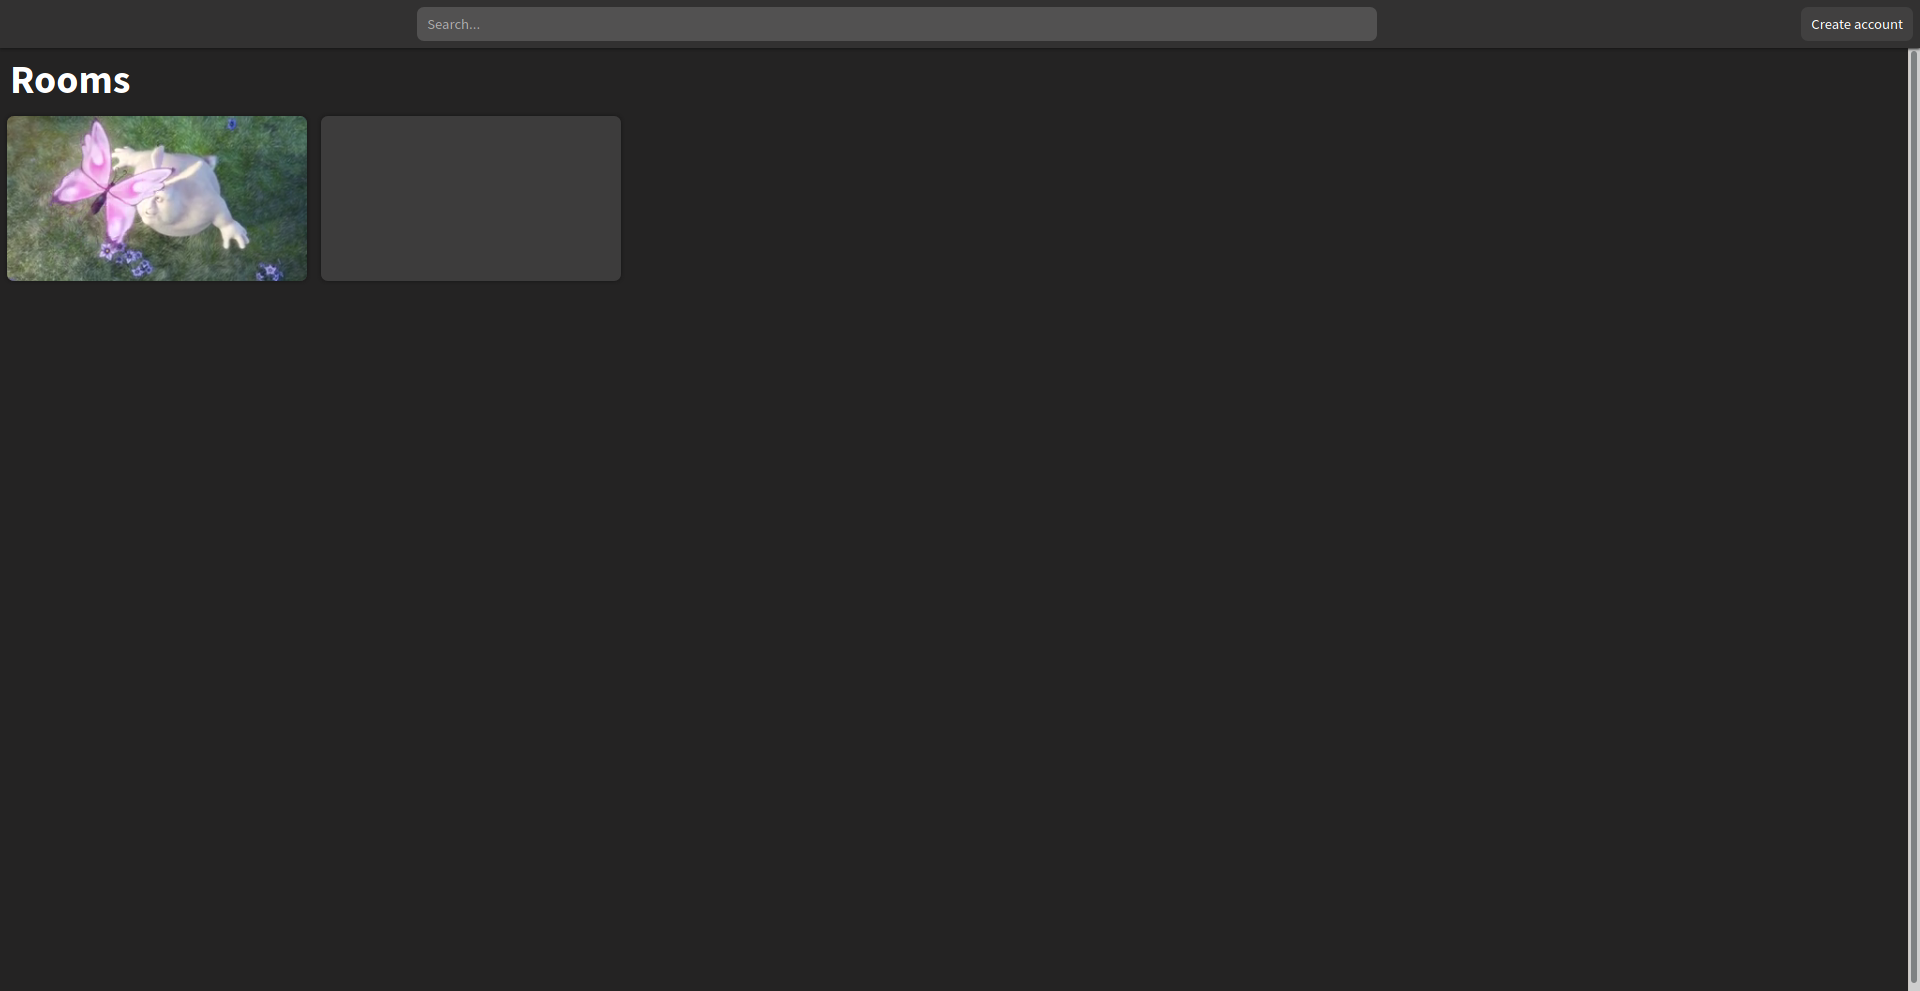
\includegraphics[scale=0.24]{main.png} 
   \caption{Главная страница приложения}
   \label{fig:arch:main_page}
\end{figure}
 
\begin{figure}[H]
 \centering
   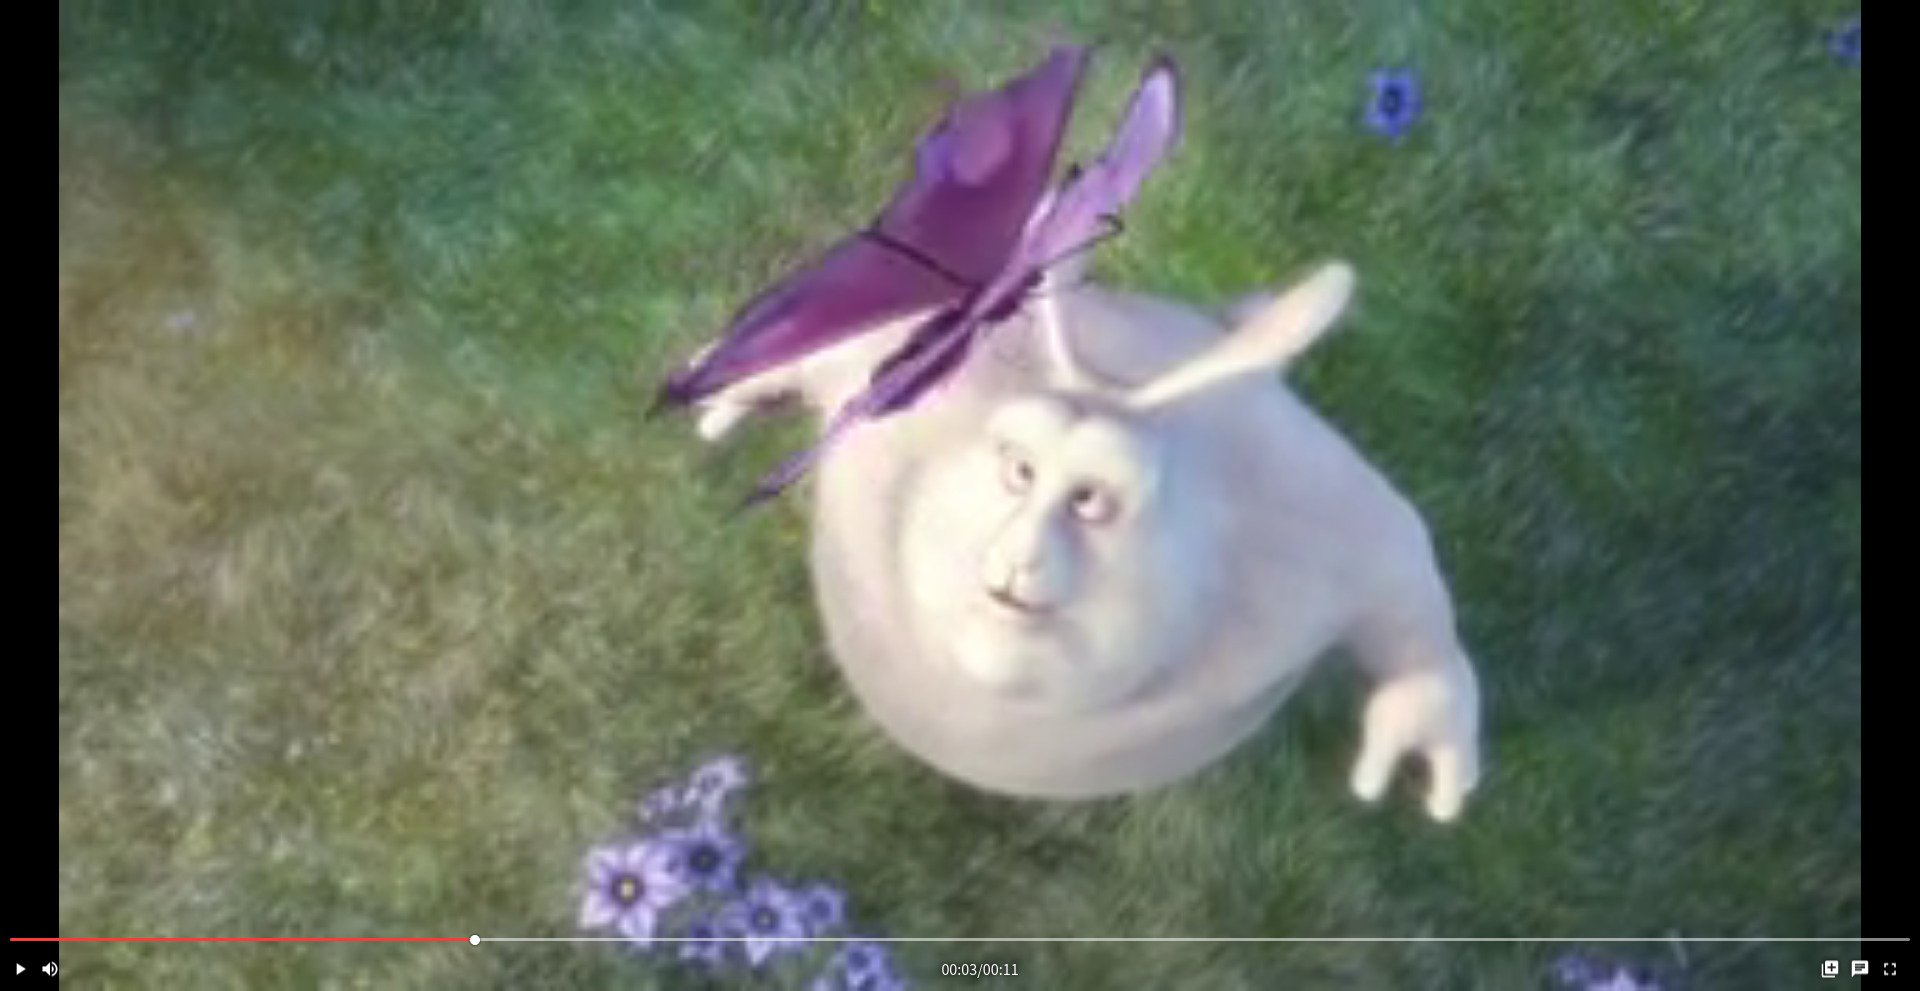
\includegraphics[scale=0.24]{room.jpg} 
   \caption{Страница комнаты}
   \label{fig:arch:room_page}
\end{figure}
 
Основная страница содержит в себе следующий набор функциональных возможностей:
\begin{itemize}
 \item авторизация пользователей;
 \item изменение пользовательских настроек;
 \item отображение доступных комнат;
 \item поиск комнат;
 \item предпросмотр комнат;
 \item переход на страницу комнаты.
\end{itemize}
 
Станица плеера имеет следующие функции:
\begin{itemize}
 \item проверка пароля комнаты;
 \item сохранение пароля при удачном вводе, чтобы пропустить его ввод в дальнейшем;
 \item воспроизведение видеоролика;
 \item остановка видеоролика;
 \item перемотка видеоролика;
 \item изменение громкости видеоролика;
 \item открытие видеоролика в полноэкранном режиме;
 \item отображение уведомлений о текущих действиях плеера;
 \item добавление видеоролика в список воспроизведения;
 \item добавление нескольких роликов в список воспроизведения;
 \item удаление ролика из списка воспроизведения;
 \item удаление всех роликов из списка воспроизведения;
 \item выбор следующего ролика для воспроизведения из списка воспроизведения;
 \item автоматическое включение следующего ролика из списка воспроизведения;
 \item синхронизация времени ролика между пользователями текущей комнаты;
 \item синхронизация состояния воспроизведения между пользователями текущей комнаты;
 \item синхронизация источника текущего видеоролика между пользователями текущей комнаты;
 \item отправка и получение сообщений в чате комнаты.
\end{itemize}
 
\subsection{Учётная запись пользователя}
Для работы пользователя с веб-приложением необходимо иметь учетную запись. Каждый пользователь при первом открытии страницы приложения автоматически получает учетную запись без необходимости ввода каких-либо данных. Данная учетная запись имеет статус анонимной. Это сделано для того чтобы любой пользователь мог сразу начать пользоваться сервисом. Пользователи с анонимной учетной записью имеют ряд ограничений:
\begin{itemize}
 \item невозможно создать собственную комнату;
 \item невозможно сменить имя пользователя;
\end{itemize}
 
Для того чтобы избавиться от ограничений пользователю необходимо создать собственную учетную запись. Для этого ему необходимо предоставить адрес электронной почты, выбрать имя пользователя и пароль (для подтверждения пароля пользователь должен ввести его два раза). 
В дальнейшем пользователь при посещении сайта будет сразу использовать созданную им учетную запись.
Для сохранения пользовательской информации в рамках текущей сессии, она записывается в хранилище состояний, предоставленный JavaScript библиотекой Redux.
 
\subsection{Список комнат}
Каждый пользователь имеет возможность просмотра списка комнат на главной странице. Данные для данного списка загружаются из базы данных и автоматически обновляются при их изменении.
Также пользователь имеет возможность производить поиск комнат, для этого имеется строка поиска в верхней части страницы.
 
Список комнат представлен в виде набора плиток. На данных плитках находится основная информация о данной комнате: название, защищённость паролем, а также окно предпросмотра текущего видеоролика. 
При нажатии на плитку комнаты пользователь перенаправляется на страницу данной комнаты. 

\subsection{Комната}
Перед тем как получить доступ к комнате происходит дополнительная проверка. 
Если комната защищена паролем, то пользователь сначала попадает на страницу с формой для ввода пароля. 
В случае ввода неправильного пароля пользователь получает уведомление об ошибке и ему предлагается ввести пароля снова. 
При вводе верного пароля, он сохраняется в локальном хранилище браузера для повторного использования и пользователь получает доступ к комнате. 

\subsection{Варианты использования}
Далее будут рассмотрены основные варианты использования разработанного веб-приложения.

\subsubsection{ВИ Создание учётной записи}~\par
\label{use:reg}
Описание ВИ: Пользователь имеет возможность при желании создать личную учётную запись.
 
Предусловия основного потока действий нет.
 
Основной поток действий:
\begin{itemize}
   \item пользователь нажимает кнопку "Create account";
   \item пользователь вводит электронную почту, имя пользователя, пароль и подтверждение пароля.
\end{itemize}
 
Ограничения: различные ограничения, установленные провайдером аутентификации Firebase.
 
\subsubsection{ВИ Использование своей учётной записи}~\par
Описание ВИ: Пользователь имеет возможность использовать личную учётную запись.
 
Предусловия основного потока действий: у пользователя имеется учётная запись см.~\ref{use:reg}.
 
Основной поток действий:
\begin{itemize}
   \item пользователь нажимает кнопку "Create account";
   \item пользователь нажимает кнопку "Existing user";
   \item пользователь вводит электронную почту и пароль.
\end{itemize}
 
Ограничения: различные ограничения, установленные провайдером аутентификации Firebase.

\subsubsection{ВИ Создание комнаты}~\par
\label{use:roomcreate}
Описание ВИ: Пользователь имеет возможность создать комнату для совместного просмотра.
 
Предусловия основного потока действий: пользователь должен быть авторизован.
 
Основной поток действий:
\begin{itemize}
   \item пользователь нажимает кнопку "Create";
   \item пользователь вводит название комнаты и пароль;
   \item клиент получает список комнат и обновляет интерфейс.
\end{itemize}
 
Ограничения: имя комнаты должно быть непустой строкой.
 
\subsubsection{ВИ Поиск комнаты}~\par
Описание ВИ: Пользователь имеет возможность искать комнату по её имени для совместного просмотра.
 
Предусловия основного потока действий: Комната существует. Для создания комнаты см.~\ref{use:roomcreate}.
 
Основной поток действий:
\begin{itemize}
   \item пользователь начинает писать название комнаты;
   \item при изменении текста в строке поиска система делает поиск по имени комнаты;
   \item клиент получает список комнат и обновляет свой интерфейс.
\end{itemize}
 
Ограничения: имя комнаты должно быть непустой строкой.

\subsubsection{ВИ Подключение к комнате}~\par
\label{use:join}
Описание ВИ: Пользователь имеет возможность присоединиться к комнате для совместного просмотра.
 
Предусловия основного потока действий: комната должна существовать см.~\ref{use:roomcreate}.
 
Основной поток действий:
\begin{itemize}
   \item пользователь нажимает кнопку плитку комнаты из списка;
   \item пользователь перенаправляется на страницу комнаты.
\end{itemize}
 
Ограничения: при наличии у комнаты пароля пользователь должен ввести его, для подключения.
 
\subsubsection{ВИ Управление видеоплеером}~\par
Описание ВИ: Пользователь имеет возможность управлять видеоплеером комнаты во время совместного просмотра.
 
Предусловия основного потока действий: комната должна существовать см.~\ref{use:roomcreate}, Пользователь присоединен к комнате см.~\ref{use:join}.
 
Основной поток действий:
\begin{itemize}
   \item Пользователь имеет следующие опций для управления плеером: запуск и остановка воспроизведения видео, перемотка, настройка громкости, открытие полноэкранного режима.
\end{itemize}
 
Ограничения: Для взаимодействия с плеером должно быть выбрано видео для воспроизведения см.~\ref{use:addvideo}.
 
\subsubsection{ВИ Добавление видео по ссылке}~\par
\label{use:addvideo}
Описание ВИ: Пользователь имеет возможность добавить видео в список воспроизведения комнаты для совместного просмотра.
 
Предусловия основного потока действий: комната должна существовать см.~\ref{use:roomcreate}, Пользователь присоединен к комнате см.~\ref{use:join}.
 
Основной поток действий:
\begin{itemize}
   \item пользователь открывает меню списка воспроизведения;
   \item пользователь нажимает кнопку "Add";
   \item пользователь вводит ссылку на ролик в строку поиска;
   \item клиент получает список видео и обновляет интерфейс;
   \item пользователь нажимает кнопку "Add" у нужного видеоролика.
\end{itemize}
 
Ограничения: ссылка должна поддерживаться приложением.
 
\subsubsection{ВИ Удаление видео из списка воспроизведения}~\par
Описание ВИ: Пользователь имеет возможность удалить видео в список воспроизведения комнаты для совместного просмотра.
 
Предусловия основного потока действий: комната должна существовать см.~\ref{use:roomcreate}, Пользователь присоединен к комнате см.~\ref{use:join}, в списке воспроизведения должны быть видеоролики см.~\ref{use:addvideo}.
 
Основной поток действий:
\begin{itemize}
   \item пользователь открывает меню списка воспроизведения;
   \item пользователь нажимает кнопку "крестик" у необходимого видеоролика.
\end{itemize}
 
Альтернативный поток действий:
\begin{itemize}
   \item пользователь открывает меню списка воспроизведения;
   \item пользователь нажимает кнопку "Reset".
\end{itemize}
 
Ограничений нет.
 
\subsubsection{ВИ Использование чата}~\par
Описание ВИ: Пользователь имеет возможность общаться с другими пользователями, используя текстовый чат.
 
Предусловия основного потока действий: комната должна существовать см.~\ref{use:roomcreate}, Пользователь присоединен к комнате см.~\ref{use:join}.
 
Основной поток действий:
\begin{itemize}
   \item пользователь открывает текстовый чат;
   \item пользователь вводит сообщение в текстовое поле;
   \item пользователь нажимает кнопку "Send" или клавишу Enter.
\end{itemize}
 
Ограничения: сообщение должно быть непустой строкой.

\subsection{Тестирование приложения}
 
Для проведения тестирования веб-приложения использовалось ПО из проекта Selenium. 
В рамках данного проекта разработан набор различных программ, которые помогают автоматизировать процесс тестирования веб-приложений. 
Для данного проекта использовался Selenium WebDriver - универсальный интерфейс для взаимодействия с драйвером браузера, веб-браузер Firefox и драйвер geckodriver. 
Для проведения тестов использовалась библиотека для языка Python и расширение для браузера Firefox~--- Selenium IDE.
 
Также было проведено ручное тестирование механизма синхронизации, так как при помощи Selenium их протестировать затруднительно. 
В рамках ручного тестирования было проведено дымовое тестирование возможностей видеоплеера и механизмов синхронизации.
